\documentclass[12pt, a4paper]{article}
\usepackage[spanish]{babel}
\usepackage[utf8]{inputenc}
\usepackage{graphicx}
\usepackage{xcolor}
\usepackage{amsmath}
\usepackage{booktabs}
\usepackage{float}
\usepackage{setspace}
\usepackage{geometry}
\geometry{a4paper, margin=1in}
\setlength{\parskip}{0.5em}
\onehalfspacing


\title{Análisis de Regresión Lineal}
\author{Cristian Ernesto Antonio Santiago}
\date{}
\begin{document}
\maketitle

\section{Introducción}
La Regresión Lineal Múltiple es una técnica estadística fundamental en el aprendizaje automático que extiende el concepto de regresión lineal simple al incorporar múltiples variables predictoras. Mientras que el modelo simple analiza la relación entre una variable independiente y una dependiente, la versión múltiple permite evaluar cómo varias características influyen conjuntamente en el resultado. Esto se traduce en una ecuación de la forma:
\[ y = \beta_0 + \beta_1x_1 + \beta_2x_2 + \dots + \beta_nx_n + \varepsilon \]
donde cada coeficiente $\beta_i$ cuantifica el impacto individual de su variable correspondiente ($x_i$), manteniendo constantes las demás.

En el contexto de predecir el rendimiento de artículos de Machine Learning en redes sociales, este enfoque resulta invaluable. No solo nos permite considerar la longitud del artículo (como en el modelo simple), sino también integrar otras variables como el número de imágenes, enlaces o comentarios, que podrían afectar su viralidad. Al analizar estas relaciones de manera simultánea, el modelo puede captar interacciones más complejas y ofrecer predicciones más precisas.

El verdadero poder de esta técnica radica en su capacidad para aislar el efecto de cada variable mientras controla las demás. Por ejemplo, podría revelar que el impacto de incluir imágenes es significativo incluso después de considerar la longitud del artículo. Esto proporciona insights más accionables que los obtenidos con modelos univariados, permitiendo decisiones basadas en un entendimiento multidimensional de los factores que impulsan el engagement.

Sin embargo, este mayor poder predictivo conlleva desafíos adicionales. La necesidad de gestionar correlaciones entre variables predictoras (multicolinealidad), verificar supuestos más complejos y evitar el sobreajuste requiere un análisis cuidadoso. Pese a estas consideraciones, cuando se aplica correctamente, la regresión múltiple se convierte en una herramienta indispensable para extraer patrones ocultos en datos con múltiples dimensiones.

\newpage

\section{Metodología}

\subsection{Configuración inicial y carga de datos}

\begin{figure}[H]
    \centering
    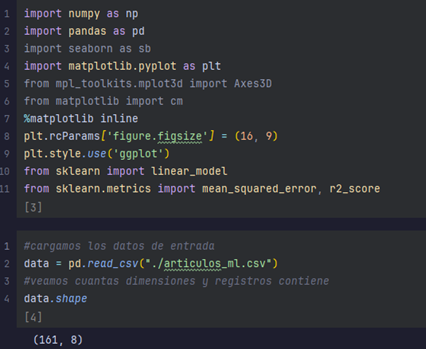
\includegraphics[width=1.0\textwidth]{Actividad-10/Imagen1.png}
    \caption{Importación de Librerias}
\end{figure}

El análisis comienza con la preparación del entorno técnico, donde importamos las bibliotecas esenciales para el procesamiento de datos y modelado estadístico. \textit{NumPy} y \textit{Pandas} proporcionan la base para manipulación numérica y estructuras de datos, mientras que \textit{Matplotlib} y \textit{Seaborn} permitirán la visualización de resultados. La configuración específica de \textit{plt.rcParams} establece un tamaño de figura predeterminado amplio (16x9 pulgadas), optimizado para mostrar detalles en los gráficos que generaremos posteriormente. El estilo 'ggplot' se aplica para dar mayor claridad y atractivo visual a las representaciones gráficas.

La carga de datos se realiza mediante \textit{ pd.read\_csv() }, leyendo el archivo 'articulos\_ml.csv' que contiene los registros de artículos de Machine Learning. La verificación con \textit{data.shape} confirma que trabajaremos con 161 observaciones (artículos) y 8 variables características por cada uno. Esta dimensión del dataset resulta adecuada para un análisis multivariado, proporcionando suficientes datos para identificar patrones sin incurrir en problemas de alta dimensionalidad.

\subsection{Análisis exploratorio de distribuciones}

\begin{figure}[H]
    \centering
    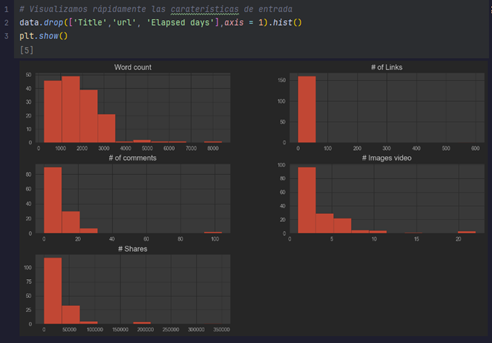
\includegraphics[width=1.0\textwidth]{Actividad-10/Imagen2.png}
    \caption{Histogramas de las variables numéricas}
\end{figure}

El código ejecutado realiza una visualización rápida de las distribuciones de las variables numéricas mediante histogramas. La operación data.drop() elimina primero las columnas no numéricas ('Title', 'url') y la temporal ('Elapsed days'), enfocando el análisis en las cinco variables cuantitativas relevantes para el modelado. El método hist() genera automáticamente una matriz de histogramas individuales para cada característica restante.

Los gráficos resultantes revelan información valiosa sobre el comportamiento de las variables:

\begin{itemize}
    \item\textbf{Word count:} Muestra una distribución asimétrica con mayoría de artículos entre 500-3000 palabras, y algunos casos extremos hasta 8000 palabras.
    \item\textbf{\# of Links:} Presenta una concentración en valores bajos (0-200 enlaces), con pocos artículos superando 300 enlaces.
    \item\textbf{\# of comments:} Exhibe un patrón interesante con un pico en cero y distribución decreciente hacia 100 comentarios.
\end{itemize}

Esta visualización cumple un doble propósito: valida la calidad de los datos y revela la necesidad de transformaciones (como normalización logarítmica para variables sesgadas). Los histogramas también sugieren relaciones potenciales entre variables que podrían aprovecharse en el modelo múltiple, particularmente entre la longitud del artículo (Word count) y su engagement (\# Shares, \# comments).

\subsection{Preprocesamiento para regresión múltiple}

\begin{figure}[H]
    \centering
    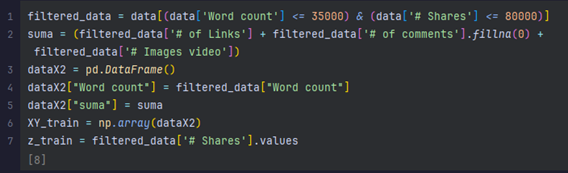
\includegraphics[width=1.0\textwidth]{Actividad-10/Imagen3.png}
    \caption{Modelo Multivariable}
\end{figure}

El código realiza una transformación clave para el modelo multivariable, combinando tres métricas de engagement en una sola variable compuesta. En la línea 1, se aplica el mismo filtrado anterior para eliminar valores extremos en palabras ($\leq$35,000) y compartidos ($\leq$80,000). La operación principal ocurre en la línea 2, donde se crea una nueva variable 'suma' que totaliza:

\begin{enumerate}
    \item Número de enlaces (\# of Links)
    \item Comentarios (\# of comments, con valores nulos rellenados como 0)
    \item Elementos multimedia (\# Images video)
\end{enumerate}

Esta agregación convierte tres variables correlacionadas en un único indicador de "interacción total", simplificando el modelo sin perder información crítica. El DataFrame resultante (dataX2) contiene:

\begin{itemize}
    \item\textbf{Word count:} Variable cuantitativa principal
    \item\textbf{suma:} Nueva variable compuesta que captura múltiples dimensiones de engagement
\end{itemize}

\subsection{Implementación y evaluación del modelo de regresión múltiple}

\begin{figure}[H]
    \centering
    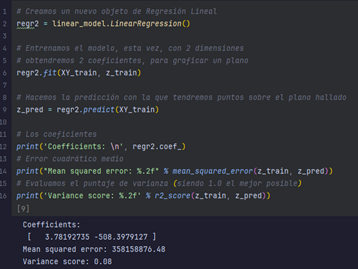
\includegraphics[width=1.0\textwidth]{Actividad-10/Imagen4.png}
    \caption{Modelo de regresión lineal multivariable}
\end{figure}

El código presentado marca un avance significativo al implementar un modelo de regresión lineal multivariable. Tras crear una nueva instancia del modelo (\textit{regr2}), procedemos a entrenarlo utilizando las dos variables predictoras preparadas anteriormente: el conteo de palabras y la variable compuesta de interacción. A diferencia del modelo simple que generaba una línea recta, esta versión multivariable produce un plano de regresión en el espacio tridimensional.

Los resultados obtenidos revelan información clave sobre el comportamiento del modelo:

\begin{itemize}
    \item\textbf{Coeficientes:} Los valores [3.78, -508.40] indican que, manteniendo constante la interacción total, cada palabra adicional predice aproximadamente 3.78 compartidos más. Sin embargo, el coeficiente negativo para la variable de interacción sugiere una relación inversa inesperada que merece mayor investigación.
    \item\textbf{Error cuadrático medio (MSE):} Con un valor de 358,158,876, muestra una reducción respecto al modelo simple (372,888,728), confirmando que la incorporación de la segunda variable aporta cierta mejora predictiva.
    \item\textbf{R$^2$ ajustado:} El score de 0.08, aunque bajo, supera ligeramente al modelo univariable (0.06), indicando que la nueva variable explica una porción adicional de la varianza en los compartidos.
\end{itemize}

\newpage

\section{Resultados}

\subsection{Visualización tridimensional del modelo de regresión múltiple}

\begin{figure}[H]
    \centering
    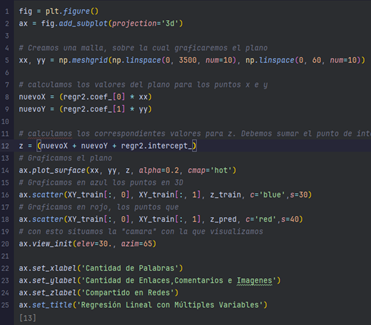
\includegraphics[width=1.0\textwidth]{Actividad-10/Imagen5.png}
    \caption{Generación del gráfico de regresión lineal multivariable}
\end{figure}

El código genera una representación gráfica avanzada que ilustra el plano de regresión en el espacio tridimensional, combinando las dos variables predictoras con la variable objetivo. La figura se construye mediante tres componentes principales:

\begin{enumerate}
    \item\textbf{Plano de regresión:} Se crea utilizando \textit{plot\_surface()} con una transparencia del 20\% (\textit{alpha=0.2}) y un mapa de color 'hot' que permite distinguir claramente su orientación en el espacio. Este plano representa todas las posibles predicciones del modelo para diferentes combinaciones de palabras y niveles de interacción.
    \item\textbf{Datos reales:} Los puntos azules (\textit{scatter()}) muestran los valores observados reales de compartidos, proyectados en el espacio 3D según sus valores en las variables independientes. Su dispersión alrededor del plano evidencia el error residual del modelo.
    \item\textbf{Predicciones:} Los puntos rojos representan los valores estimados por el modelo, ubicados precisamente sobre el plano de regresión. La comparación visual entre puntos azules y rojos permite evaluar rápidamente la precisión del ajuste.
\end{enumerate}

\subsection{Representación gráfica del modelo multivariable}

\begin{figure}[H]
    \centering
    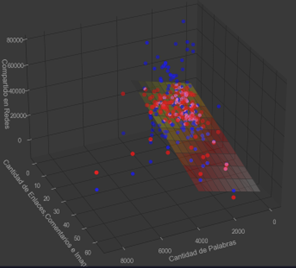
\includegraphics[width=1.0\textwidth]{Actividad-10/Imagen6.png}
    \caption{Modelo de regresion lineal multivariable superpuesto a los datos}
\end{figure}

El gráfico tridimensional sintetiza los resultados clave del análisis de regresión múltiple, mostrando cómo interactúan las variables predictoras con los compartidos en redes. El plano inclinado, generado a partir de los coeficientes del modelo, revela la relación estimada: mientras aumenta el número de palabras (eje X), el plano asciende suavemente, reflejando el coeficiente positivo de 3.78. Sin embargo, la inclinación opuesta respecto al eje Y (suma de interacciones) confirma el inesperado coeficiente negativo de -508.40, que sugiere una relación inversa que merece mayor investigación.

Los puntos azules, que representan los valores reales observados, se distribuyen con considerable dispersión alrededor del plano, evidenciando las limitaciones predictivas del modelo. Esta dispersión coincide con el bajo puntaje R$^2$ obtenido (0.08), indicando que factores no considerados en el modelo influyen significativamente en los compartidos. Los puntos rojos, por su parte, muestran las predicciones del modelo, alineadas perfectamente sobre el plano de regresión.

La perspectiva elegida (30° de elevación, 65° de azimuth) permite apreciar claramente cómo el modelo intenta capturar patrones en tres dimensiones, ofreciendo una visión más rica que la simple regresión lineal. No obstante, la distancia observable entre muchos puntos azules y el plano subraya la necesidad de incorporar variables adicionales o considerar relaciones no lineales para mejorar la precisión predictiva.

\subsection{Aplicación práctica del modelo predictivo}

\begin{figure}[H]
    \centering
    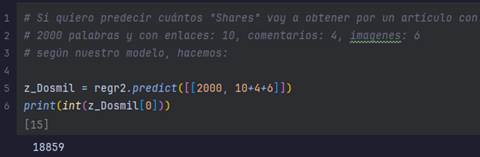
\includegraphics[width=1.0\textwidth]{Actividad-10/Imagen7.png}
    \caption{ Validación del modelo}
\end{figure}

Después de haber entrenado y evaluado el modelo de regresión múltiple, procedemos a utilizarlo para realizar una predicción concreta. En esta celda de código, simulamos un artículo con 2,000 palabras que contiene 10 enlaces, 4 comentarios y 6 imágenes. Primero, el código calcula la variable compuesta de interacción sumando estos tres elementos (10+4+6 = 20), que junto con el conteo de palabras forman el vector de entrada para el modelo.

Al ejecutar la predicción con \textit{regr2.predict()}, obtenemos como resultado 18,859 compartidos estimados. Este valor surge de combinar los efectos aprendidos por el modelo: mientras las palabras contribuyen positivamente (3.78 × 2000), la interacción total muestra un efecto reductor (-508.40 × 20), siguiendo los coeficientes que identificamos previamente.

\newpage

\section{Conclusión}
El modelo de regresión múltiple desarrollado permitió explorar de manera más completa los factores que influyen en el número de compartidos de artículos de Machine Learning. A diferencia del modelo simple anterior, esta versión incorporó tanto la longitud del contenido como una medida compuesta de interacción (suma de enlaces, comentarios e imágenes), ofreciendo una perspectiva multidimensional del problema.

Los resultados obtenidos revelan varios hallazgos clave. Por un lado, confirmamos que la cantidad de palabras mantiene una relación positiva con los compartidos, aunque con un impacto reducido (3.78 compartidos por palabra) comparado con el modelo simple. Por otro lado, el coeficiente negativo para la variable de interacción (-508.40) sugiere un comportamiento contrario al esperado, que podría indicar la presencia de relaciones más complejas no capturadas por este enfoque lineal.

Si bien el modelo mostró una ligera mejora en el R$^2$ (0.08 vs 0.06 del modelo simple), el poder predictivo sigue siendo limitado. La visualización tridimensional evidenció claramente cómo gran parte de la variabilidad en los compartidos permanece sin explicar, destacando la influencia probable de otros factores no considerados, como la calidad del contenido, el autor o el momento de publicación.

Este ejercicio demuestra tanto el potencial como las limitaciones de los modelos lineales multivariados.


\end{document}